%\documentclass[12pt,xcolor=dvipsnames,mathserif]{beamer}
\documentclass[12pt,xcolor=dvipsnames,handout,mathserif,aspectratio=169]{beamer}

\usepackage{hyperref}

\usepackage{pgfpages}
%\pgfpagesuselayout{2 on 1}[border shrink=2.5mm]
%\pgfpageslogicalpageoptions{1}{border code=\pgfusepath{stroke}}
%\pgfpageslogicalpageoptions{2}{border code=\pgfusepath{stroke}}


% Specify theme
%\usetheme{Madrid}
\usetheme{Boadilla}
% See deic.uab.es/~iblanes/beamer_gallery/index_by_theme.html for other themes

% Specify base color
%\usecolortheme[named=OliveGreen]{structure}
\usecolortheme[named=RoyalBlue]{structure}
% See http://goo.gl/p0Phn for other colors

% Specify other colors and options as required
\setbeamercolor{alerted text}{fg=Red}
\setbeamertemplate{items}[square]

% Specify some useful short commands
\newcommand{\bbl}[1]{{\color{NavyBlue} \textbf{#1}}}
\newcommand{\bre}[1]{{\color{red} \textbf{#1}}}
\newcommand{\bgr}[1]{{\color{PineGreen} \textbf{#1}}}
\newcommand{\un}{\texttt{\char`_}}


% Title and author information
\title[Introductory Statistics with Excel]{Introductory Statistics with Excel}
\author[Andrew Parnell]{Andrew Parnell}
\institute[UCD]{University College Dublin \begin{center} 
\includegraphics[width=1.5cm]{UCDlogo.pdf}\end{center} }
\date[Class 2]{Class 2 - Experimental Design and probability}
%\date{Lecture 2 -- part 1}

\begin{document}

\titlepage

\begin{frame}{Learning outcomes}

In this class we will cover
\begin{itemize}
\item Experimental design
\item Randomised controlled trials
\item Confounding
\item Observational studies
\item An introduction to the normal distribution
\end{itemize}

\end{frame}



\begin{frame}{Obtaining data from experiments and observational studies}

Sometimes we have the ability to design an \bgr{experiment} (or \bgr{trial}) that enables us to answer specific questions of interest. In such cases, we might be able to determine the \bbl{cause and effect} relationship between variables.\\
\pause
\vspace{0.2cm}
In this class we will meet \bgr{Randomised Controlled Trials (RCTs)}, possibly the most important idea in science!\\
\pause
\vspace{0.2cm}
When an experiment is not possible, we might run an \bbl{observational study}
\end{frame}

\begin{frame}{ The general problem }

\begin{block}{}
Suppose I have a pill which is hypothesised to cure a particular disease. I give the pill to an animal and it recovers from the disease. How do I know whether the pill caused it to recover from the disease? Suppose it had not recovered from the disease. Do I then know that the pill hasn't worked?
\end{block}

\end{frame}


\begin{frame}{Types of research studies}

\begin{description}
\item[Observational studies] occur when researchers simply observe (or collect data via e.g. a survey) the participants about behaviour. For example we may run an observational study in which we record the blood pressure and frequency of milking for a number of cows.
\pause
\item[Experiments] occur when researchers manipulate one or more variables with the possibility of affecting some particular outcome of interest. For example, the researchers might forcefully change the number of milkings and then record their blood pressure
\end{description}
\pause
It is only in the second situation that we can really determine whether number of milkings has an effect on blood pressure
\end{frame}

\begin{frame}{Explanatory and response variables }

Most experiments are run because we want to determine the relationship between two or more variables. The `cause' variable is known as the \bbl{Explanatory variable} and the `effect' variable is known as the \bgr{Response variable}. In the previous example, frequency of milking is the explanatory variable and blood pressure is the response variable. 

\begin{block}{}
Which are the explanatory/response variables in the following situations?
\begin{itemize}
\pause
\item \bgr{Whether taking aspirin or not} and \bbl{cholesterol level}
\pause
%\item \bgr{Level of education} and \bbl{level of education of parents}
\pause
\item \bgr{Likelihood of voting for the Green party} and \bbl{agreement with statement `humans are responsible for global warming'}
\end{itemize}
\end{block}

\end{frame}

\begin{frame}{Problems in observational studies: confounding variables}

\begin{block}{Example 1}
A recent study showed that people who drink red wine tend to live longer than those who do not drink red wine. The study concluded that red wine might have beneficial health effects
\end{block}
\pause
\begin{block}{Example 2}
Another study found that people who wore their shoes to bed tended to wake up with a headache. They concluded that wearing shoes to bed might be detrimental to a person's health 
\end{block}
\pause
In both these cases a \bre{confounding (or lurking) variable} is present that affects both the response and explanatory variables and casts doubt on the causal link between them
\end{frame}

\begin{frame}{Confounding variables: the solution }

We can remove the influence of confounding variables by conducting an experiment where we randomly assign people to different groups.
\begin{itemize}
\item In example 1, we could randomly assign people to one of several \bgr{treatment groups}: e.g. no red wine, 1-2 glasses of red wine per day, 3+ glasses of red wine per day. We could then follow up how long they live over several years and determine the health benefits of red wine
\pause
\item In example 2, we could randomly assign people to the treatment groups: wear shoes to bed, do not wear shoes to bed. We could then record how often the people in the two groups woke up with a headache
\end{itemize}
\pause
This \bbl{experimental design} works because we are breaking the confounding variable's control over the response and explanatory variables

\end{frame}

\begin{frame}[fragile]{}
\bbl{\Huge Randomised Controlled Trials}\\ 
\vspace{0.5cm}
\end{frame}


\begin{frame}{Designing a good experiment }

There are a few things that generally make a good experiment:
\begin{itemize}
\item \bbl{Randomisation} (randomly allocating subjects to different groups) lessens the effect of any confounding variables. The benefit of randomisation is that each of the treatment groups should be roughly equivalent aside from the explanatory variable
\item \bbl{Blocking} Grouping variables over which we have control over into categories
\item \bbl{A control group} which receives no treatment (or a dummy treatment) allows us to compare the true effect on the response variable had no treatment occurred
\item \bbl{Blinding} in which neither the subject nor the researcher knows which treatment is being applied. This is particularly important in medical studies
\end{itemize}

\end{frame}

\begin{frame}{Control groups and placebos }

\begin{itemize}
\item We use a control group to determine whether the change in response is due to the treatment or not. For example, it is well-known that people recover from coughs and colds without any treatment at all given enough time. A treatment should thus only prove acceptable if it can reduce the amount of time people are sick
\pause
\item A \bre{placebo} is a dummy treatment that is identical in every way from the normal treatment except that of the active ingredient. For example, a sugar pill of exactly the same colour and shape to the pill being tested for medical reasons is often given to a placebo group 
\end{itemize}

\end{frame}

\begin{frame}{The remarkable placebo effect }

\begin{itemize}
\item It is well known that giving someone a placebo will tend to improve the response variable more than giving them no treatment at all
\pause
\item Remarkably, it has also been shown that green sugar pills are better than red sugar pills for treating anxiety. Similarly, a salt-water placebo injection was found to be more effective than a standard white sugar pill
\pause
\item Even more strangely, in the 1950s a placebo operation was found to be a more effective treatment for Angina than the real operation it was replacing
\end{itemize}
\pause
The placebo effect is not fully understood in science and remains an active area of research. %See Dr Ben Goldacre's website \url{www.badscience.net} for more information about placebos
\end{frame}

\begin{frame}{Blinding }

\begin{block}{}
Suppose you are running an experiment into a potential cure for a serious disease. For each person who arrives in your office you must allocate them to either the proper treatment or a placebo. A very sick looking person arrives into your office. Do you allocate them to the treatment or placebo?
\end{block}
\pause
\begin{block}{}
You are taking part in a trial to see whether paracetemol or ibuprofen is better for reducing headaches. You have been allocated to the aspirin group but you really don't like aspirin and far prefer taking ibuprofen
\end{block}
\pause
In both these situations it is beneficial for the experimenter and the subjects not to know whether they are receiving the treatment or placebo. If only the experimenter knows which treatment you are taking it is known as \bbl{single blinding}. If neither the experimenter nor the subject know it is called \bgr{double blinding}

\end{frame}

\begin{frame}{ Randomised controlled trials: the gold standard }

%The best RCTs will include the following:
%\small
\begin{enumerate}
\item Take a \bbl{large sample} of the population of interest. A large sample will be more representative of the population.
\pause
\item \bbl{Randomly allocate} each person in each block to either receiving the \bbl{treatment} or a \bbl{placebo} (or the current best treatment). The randomisation will lessen the effect of confounding variables. The placebo will allow the measurement to focus only on the effect of the treatment and not the action of being treated
\pause
\item Make sure that neither the experimenters nor the subjects know to which group they have been allocated. This \bbl{double blinding} will stop subjects/experimenters biasing the response to the treatment
\pause
\item Record your response variable(s) of interest and report the \bbl{difference} in the response variable(s) between the treatment group and the placebo group
\end{enumerate}
%\normalsize
\pause
The above is remarkably simple and incredibly powerful yet almost completely unknown to the general public
\end{frame}


\begin{frame}{ Some other useful things to know }

\begin{itemize}
\item It is often the case that RCTs use volunteers. Those who volunteer early in the study might be fitter or more optimistic. It is therefore best to randomise the order to which they are allocated to treatment/placebo
\pause
\item If the subjects are undergoing more than one treatment (e.g. two different drugs) it is usually best to randomise the order of the treatments, to leave a gap between their administration, or to give them both simultaneously
\pause
\item In some situations (e.g. physiotherapy) it is very hard to find good placebos. Finding a good placebo requires imagination and creativity. See for example the studies in Acupuncture
\end{itemize}

\end{frame}

\begin{frame}{ Extending RCTs }

\begin{itemize}
\item If we know in advance that there will be a strong confounding variable, for example age or income, we might divide up our sample into \bbl{blocks} representing different groups of this variable. Within each group we would then randomly allocate to treatment or placebo
\pause
\item A specific example of this is a \bbl{matched pair} design whereby subjects are paired together based on equality of some important variable. We then randomly allocate one to placebo and one to response
\pause
\item If we have the resources we may make more than one measurement on each subject. This will enable us to see whether each subject responds similarly to the same treatment or not. These are known as \bbl{replicated} or \bbl{repeated measures} experimental designs
\end{itemize}

\end{frame}

\begin{frame}{The Hawthorne and other effects }

In addition to the placebo effect, a number of other factors have been observed to affect the results of an experimental study
\begin{itemize}
\item The \bbl{Hawthorne effect} occurs when a response variable is changed simply by the manor of being in an experiment. This was first noticed in the 1920s when workers in a factory improved their output when any change was made to their working conditions
\pause
\item The \bre{Experimenter effect} occurs when the experimenter has a vested interest in the outcome of the experiment and so is likely to (unconsciously) bias the results. This effect can be lessened when the experiment is double-blinded
\pause
\item The \bgr{Nocebo} effect occurs when subjects believe the treatment will actively harm them. In such cases the subjects tend to report increased side effects and reduced effectiveness of the treatment
\end{itemize}

\end{frame}

\begin{frame}{ When would you \bre{not} use an RCT? }

The main issue with RCTs is that they are usually expensive, artificial, and occasionally unethical. Consider the following examples:
\begin{itemize}
\item We want to know whether breast-feeding or formula-feeding is most beneficial for babies' development. A standard RCT would involve telling mothers to breast-feed or formula-feed based on their allocation to treatment group
\pause
\item A new drug is available to relieve pain in the very last stages of people dying from a serious disease. The drug seems to be safe and works in various animal trials. There are no pre-existing treatments for comparison purposes
\pause
\item We want to learn whether people who are left-handed are more likely to suffer from post-traumatic stress disorder. The proportion of people who are left-handed is approximately 5\% and the proportion suffering from post-traumatic stress disorder is approximately 0.1\%
\end{itemize}
\pause
In such cases we might use an \bgr{observational study} instead

\end{frame}

\begin{frame}[fragile]{}
\bbl{\Huge Observational studies}\\ 
\vspace{0.5cm}
\end{frame}

\begin{frame}{Designing good observational studies }

There are two main types of observational study:
\begin{description}
\item[Retrospective studies] where information is obtained from the past. For example, subjects may be asked to recall their past exercising behaviour
\pause
\item[Prospective studies] where information is obtained by following subjects over a period of time. This approach is generally better as people tend to forget or mis-report their past behaviour
\end{description}
\pause
A third category (which may be part of either a retrospective or prospective study) is that of a \bbl{case-control} study, whereby pairs of subjects with similar explanatory variables are matched between categories of the response variable. 

\end{frame}

\begin{frame}{Advantages of observational/case-control studies }

\begin{itemize}
\item Case-control studies do not suffer from the \bre{unethical} aspect of RCTs. The subjects are not required to change their behaviour based on an experimenter's instructions
\pause
\item They are extremely \bgr{efficient}. Consider trying to determine whether pet birds might cause lung cancer. The RCT version would involve randomly giving people pet birds (or placebo birds!) and waiting to see whether the owner's contract lung cancer. A case control study would identify a large group of people with lung cancer and another group who have not and then ask wether or not each group owned a pet bird
\pause
\item They reduce the chance of \bre{confounders}. Like a matched-pair experimental study, confounders are reduced because we can match subjects based on important variables
\end{itemize}

\end{frame}


%\begin{frame}{Dealing with confounding variables in observational studies }
%
%Aside from case-control studies, confounding variables can be at least partially removed via the use of \bgr{statistical models}. Suppose that the response variable is called $y$, the treatment allocation $t$ and the confounding variable $c$. We could write a statistical model as:
%\begin{eqnarray*}
%y = \mbox{overall effect} +  \alpha\times t + \beta\times c + \mbox{error}
%\end{eqnarray*}
%\pause
%There are methods in statistics that allow us to estimate the size of the treatment effect $\alpha$ and the confounding variable effect $\beta$. We can thus separate out the importance of the two variables. \\
%\vspace{0.2cm}
%\pause
%One such method is called \bbl{multiple linear regression}. You will study this method in detail if you study the later course \bgr{Linear Models 2}
%
%\end{frame}
%
\begin{frame}{Not just for medicine!}

RCTs and observational studies were developed with medical studies in mind. \bbl{Since we discovered RCTs and the gold standard our life expectancies have doubled!}\\
\vspace{0.5cm}
\pause
However, their use is not just restricted to the medical field. Consider the following examples
\begin{itemize}
\item How might we design an experiment to test whether studying more subjects at primary level leads to increased achievement in later years?
\pause
\item How might we design an experiment to test whether prison or rehabilitation might improve re-offending rates of drug-related crimes?
\end{itemize}

\end{frame}

\begin{frame}[fragile]{}
\bbl{\Huge The normal distribution}\\ 
\vspace{0.5cm}
\end{frame}

\begin{frame}{ The normal distribution }

Often, when looking at histograms of data we see the same shapes re-appearing:
\begin{center}
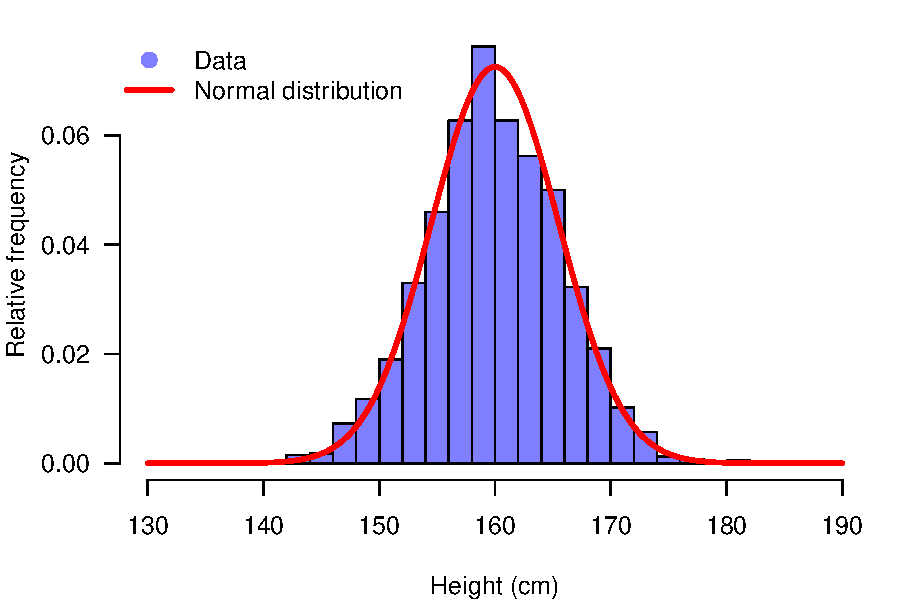
\includegraphics[width=0.5\textwidth]{WomensHeights.pdf}
\end{center}
\pause
This shape (peaked in the middle, decaying out evenly on both sides) is known as a \bgr{bell-shaped curve}. One type of these is the \bbl{normal distribution}; possibly the most important and useful probability distribution in statistics

\end{frame}

\begin{frame}{ The normal distribution and the empirical rule}

The normal distribution is very useful. If we are happy to assume that our data come from a normal distribution then we can say that:
\begin{block}{}
\begin{itemize}
\item 68.2\% of the observations will lie within 1 standard deviation of the mean
\item 95.5\% of the observations will lie within 2 standard deviations of the mean
\end{itemize}
\end{block}
\pause
\begin{columns}
\begin{column}{0.5\textwidth}
\begin{center}
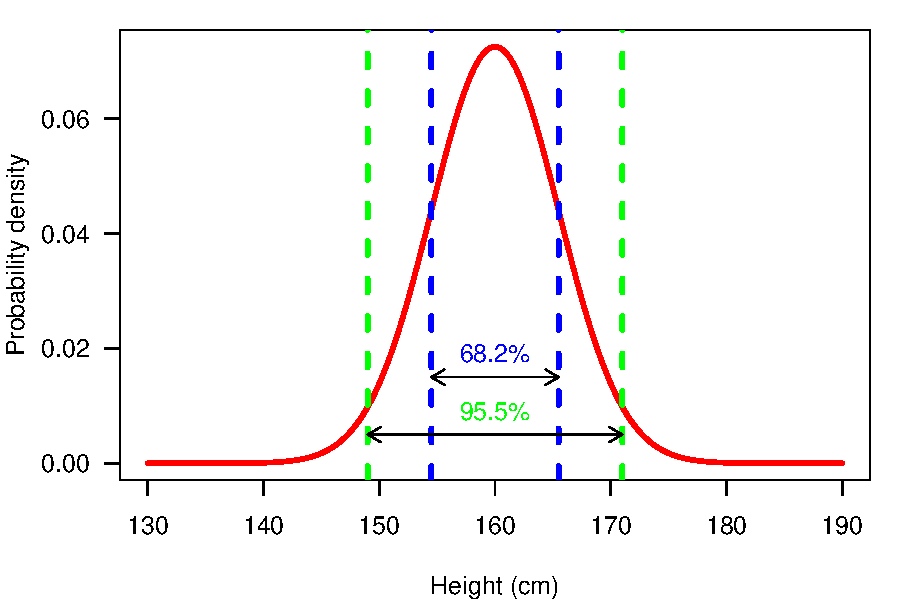
\includegraphics[width=0.9\textwidth]{NormalRule.pdf}
\end{center}
\end{column}
\pause
\begin{column}{0.5\textwidth}
We can use these facts to create predictions with uncertainty about future observations we might find.
\end{column}
\end{columns}
\end{frame}


\begin{frame}{ The normal distribution and z-scores }
\begin{itemize}
\item If we take each observation and \bgr{standardise} it by first subtracting the mean and then dividing by the standard deviation, we obtain a \bbl{$z$-score}
\pause
\item A $z$-score is useful as a relative measure of an observation in comparison to the others. The standardised observations will have mean 0 and standard deviation 1
\pause
\item If the data come from a normal distribution, then 68.2\% of the $z$-scores will lie between -1 and 1, as we know from the results on the previous slide
\pause
\item Furthermore, if a particular $z$-score is, e.g. 1.25, then we know that this value is 1.25 standard deviations away from the mean
\pause
\item We will use this trick later on when we cover \bre{hypothesis testing}
\end{itemize}
\end{frame}

\begin{frame}{Class 2 summary}
\begin{itemize}
\item Remember the key elements of an experiment: \bbl{randomisation}, \bbl{blocking}, \bbl{control groups}, \bbl{blinding}
\item The bigger the \bgr{sample size} the more precise your results will be 
\item If you can't do randomisation go for an \bbl{observational study}, but be wary of \bre{confounding}
\item The \bbl{normal distribution} and the \bgr{empirical rule} allow us to make population statements from statistics

\end{itemize}
\end{frame}


\end{document}